\section{Curvilinear Coordinates}\label{sec:other_systems}

% originally from Schoolcraft

\mtable{Cartesian Coordinates}{fig_cart_coord}{\begin{tikzpicture}[scale=3]
 % these are weirdly ordered. pay attention
 \draw[->](0,0) -- (1,0) node[right]{\scriptsize$y$};
 \draw[->](0,0) -- (0,1) node[right]{\scriptsize$z$};
 \draw[->](0,0) -- (xyz cs:z=1.5) node[right]{\scriptsize$x$};
 \draw[{\colorone}] (0,0) node[color=black,below]{\scriptsize$0$}
  -- node[pos=.5,color=black,left]{\scriptsize$x$}(xyz cs:z=1)
  -- node[pos=.5,color=black,below]{\scriptsize$y$}(1,0,1)
  -- node[pos=.7,color=black,right]{\scriptsize$z$}(1,1,1)
     node[color=black,above right]{\scriptsize$(x,y,z)$};
 \fill[{\colorone}](1,1,1) circle(.6pt);
 \draw[dashed](0,0) -- (1,0,1);
 \draw(.9,0,1)--(.9,.1,1)--(1,.1,1);
\end{tikzpicture}}

The Cartesian coordinates of a point $(x,y,z)$ are determined by following straight paths starting from the origin: first along the $x$-axis, then parallel to the $y$-axis, then parallel to the $z$-axis, as in \autoref{fig_cart_coord}. In \emph{curvilinear coordinate systems}\index{coordinates!curvilinear}, these paths can be curved. The two types of curvilinear coordinates which we will consider are cylindrical\index{coordinates!cylindrical} and spherical\index{coordinates!spherical} coordinates. Instead of referencing a point in terms of sides of a rectangular parallelepiped, as with Cartesian coordinates, we will think of the point as lying on a cylinder or sphere. Cylindrical coordinates are often used when there is symmetry around the $z$-axis; spherical coordinates are useful when there is symmetry about the origin.

\mtable{Cylindrical coordinates}{fig_cyl_coord}{\begin{tikzpicture}[scale=3]
 % these are weirdly ordered. pay attention
 \draw[->](0,0) -- (1,0) node[right]{\scriptsize$y$};
 \draw[->](0,0) -- (0,1) node[right]{\scriptsize$z$};
 \draw[->](0,0) -- (xyz cs:z=1.5) node[right]{\scriptsize$x$};
 \draw[dashed] (0,0) node[color=black,left]{\scriptsize$0$}
  -- node[pos=.5,left]{\scriptsize$x$}(xyz cs:z=1)
  -- node[pos=.5,below]{\scriptsize$y$}(1,0,1);
 \draw[{\colorone}](1,0,1) node[color=black,below right]{\scriptsize$P_0(x,y,0)$}
  -- node[pos=.7,color=black,right]{\scriptsize$z$}(1,1,1)
     node[color=black,above right]{\scriptsize$P(x,y,z)$};
 \fill[{\colorone}](1,1,1) circle(.6pt);
 \draw[dashed,{\colorone}](0,0)
  -- node[pos=.5,color=black,above right]{\scriptsize$r$} (1,0,1);
 \draw(.9,0,.9)--(.9,.1,.9)--(1,.1,1);
 \draw[->,{\colorone}](xyz cs:z=.3)
     arc[start angle=225,end angle=315,y radius=.1,x radius=.2]
     node[pos=.5,below,color=black]{\scriptsize$\theta$};
\end{tikzpicture}}

Let $P = (x,y,z)$ be a point in Cartesian coordinates in $\mathbb{R}^{3}$, and let $P_0 = (x,y,0)$ be the projection of $P$ upon the $xy$-plane. Treating $(x,y)$ as a point in $\mathbb{R}^{2}$, let $(r,\theta)$ be its polar coordinates (see \autoref{fig_cyl_coord}). Let\index{coordinates!polar} $\rho$ be the length of the line segment from the origin to $P$, and let $\phi$ be the angle between that line segment and the positive $z$-axis (see \autoref{fig_sph_coord}), which is called the \emph{zenith angle}\index{zenith angle}. Then the \textbf{cylindrical coordinates} $(r,\theta,z)$  and the \textbf{spherical coordinates} $(\rho,\theta,\phi)$ of $P(x,y,z)$ are defined as follows:\footnote{This ``standard'' definition of spherical coordinates used by mathematicians results in a left-handed system. For this reason, physicists usually switch the definitions of $\theta$ and $\phi$ to make $(\rho,\theta,\phi)$ a right-handed system.}

\mtable{Spherical coordinates}{fig_sph_coord}{\begin{tikzpicture}[scale=3]
 % these are weirdly ordered. pay attention
 \draw[->](0,0) -- (1,0) node[right]{\scriptsize$y$};
 \draw[->](0,0) -- (0,1) node[right]{\scriptsize$z$};
 \draw[->](0,0) -- (xyz cs:z=1.5) node[right]{\scriptsize$x$};
 \draw[dashed] (0,0) node[left]{\scriptsize$0$}
  -- node[pos=.5,left]{\scriptsize$x$}(xyz cs:z=1)
  -- node[pos=.5,below]{\scriptsize$y$}(1,0,1);
 \draw[dashed](1,0,1) node[below right]{\scriptsize$P_0(x,y,0)$}
  -- node[pos=.7,right]{\scriptsize$z$}(1,1,1)
     node[above right]{\scriptsize$P(x,y,z)$};
 \fill[{\colorone}](1,1,1) circle(.6pt);
 \draw[{\colorone}](0,0)--node[pos=.5,color=black,above]{\scriptsize$\rho$}(1,1,1);
 \draw[dashed](0,0) -- (1,0,1);
 \draw(.9,0,.9)--(.9,.1,.9)--(1,.1,1);
 \draw[->,{\colorone}](xyz cs:z=.3)
     arc[start angle=225,end angle=315,y radius=.1,x radius=.2]
     node[pos=.5,below,color=black]{\scriptsize$\theta$};
 \draw[->,{\colorone}](0,.2)
     arc[start angle=90,end angle=45,y radius=.2,x radius=.2]
     node[pos=.5,above,color=black]{\scriptsize$\phi$};
\end{tikzpicture}}

\keyidea{idea_cyl_coord}{Cylindrical coordinates $(r,\theta,z)$}{\mbox{}\\[-2\baselineskip]\begin{align*}
  x &= r \cos \theta & r &= \sqrt{x^2 + y^2}\\
  y &= r \sin \theta & \theta &= \tan^{-1} \left( \tfrac{y}{x} \right)\\
  z &= z & z &= z
 \end{align*}
 where $0 \le \theta \le \pi$ if $y \ge 0$ and $\pi < \theta < 2\pi$ if $y < 0$}

\keyidea{idea_sph_coord}{Spherical coordinates $(\rho,\theta,\phi)$}{\mbox{}
 \begin{align*}
  x &= \rho \sin \phi \,\cos \theta & \rho &= \sqrt{x^2 + y^2 + z^2}\\
  y &= \rho \sin \phi \,\sin \theta & \theta &= \tan^{-1} \left( \tfrac{y}{x} \right)\\
  z &= \rho \cos \phi & \phi &= \cos^{-1} \biggl( \tfrac{z}{\sqrt{x^2 + y^2 + z^2}} \biggr)
 \end{align*}
 where $0 \le \theta \le \pi$ if $y \ge 0$ and $\pi < \theta < 2\pi$ if $y < 0$
}

Both $\theta$ and $\phi$ are measured in radians. Note that $r \ge 0$, $0 \le \theta < 2\pi$, $\rho \ge 0$ and $0 \le \phi \le \pi$. Also, $\theta$ is undefined when $(x,y) = (0,0)$, and $\phi$ is undefined when $(x,y,z) = (0,0,0)$.

\example{ex_conv_coords}{Converting Between Coordinate Systems}{Convert the point $(-2,-2,1)$ from Cartesian coordinates to 1.\ cylindrical and 2.\ spherical coordinates.}{\mbox{}\\[-1.5\baselineskip]\begin{enumerate}\item $r = \sqrt{(-2)^2 + (-2)^2} = 2\sqrt{2}$ and $\theta = \tan^{-1} \left( \frac{-2}{-2} \right) = \tan^{-1}(1) = \frac{5 \pi}{4}$, since $y = -2 < 0$. Therefore  $(r,\theta,z) = \left( 2\sqrt{2},\frac{5 \pi}{4},1 \right)$.
 \item $\rho = \sqrt{(-2)^2 + (-2)^2 + 1^2} = \sqrt{9} = 3$ and $\phi = \cos^{-1} \left( \frac{1}{3} \right)
 \approx 1.23$ radians. Therefore $(\rho,\theta,\phi) = \left( 3,\frac{5 \pi}{4}, 1.23 \right)$.\eoehere
 \end{enumerate}}

For cylindrical coordinates $(r,\theta,z)$, and constants $r_0$, $\theta_0$ and $z_0$, we see from \autoref{fig:cylcoordsurf} that the surface $r = r_0$ is a cylinder of radius $r_0$ centered along the $z$-axis, the surface $\theta = \theta_0$ is a half-plane emanating from the $z$-axis, and the surface $z = z_0$ is a plane parallel to the $xy$-plane.

\begin{lxfigure}
 \flushinner{%
  \begin{tabular}{ccc}
 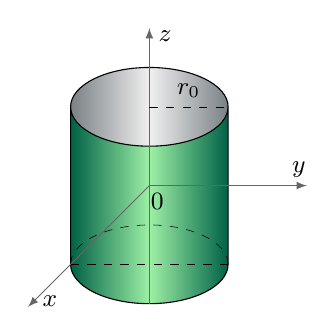
\begin{tikzpicture}
  \usetikzlibrary{arrows}
  \definecolor{insideo}{HTML}{798084}
  \definecolor{insidei}{HTML}{F0F0F0}
  \definecolor{outer}{HTML}{006146}
  \definecolor{inner}{HTML}{9EF0A6}
  \shade [left color=insideo,right color=insideo,middle color=insidei] (1,1) arc (0:180:1 and .5) --
   (-1,1) arc (180:360:1 and .5);
  \shadedraw [left color=outer,right color=outer,middle color=inner] (-1,-1) arc (180:360:1 and .5) -- (1,1) --
   (1,1) arc (360:180:1 and .5) -- (-1,-1);
  \draw (1,1) arc (0:180:1 and .5);
  \draw [dashed,line width=0.2pt] (1,-1) arc (0:180:1 and .5);
  \draw [black!60,line width=0.3pt,-latex] (0,0) -- (2,0,0);
  \draw [black!60,line width=0.3pt,-latex] (0,-1.5) -- (0,2,0);
  \draw [black!60,line width=0.3pt,-latex] (0,0) -- (0,0,4);
  \pgfputat{\pgfpointxyz{1.9}{0.2}{0}}{\pgfbox[center,center]{\small $y$}};
  \pgfputat{\pgfpointxyz{0.2}{1.9}{0}}{\pgfbox[center,center]{\small $z$}};
  \pgfputat{\pgfpointxyz{0.2}{0}{3.8}}{\pgfbox[center,center]{\small $x$}};
  \pgfputat{\pgfpointxyz{0.1}{-0.2}{0}}{\pgfbox[center,center]{\small $0$}};
  \draw [dashed,line width=0.2pt] (0,1) -- (1,1);
  \draw [dashed,line width=0.2pt] (-1,-1) -- (1,-1);
  \node [above] at (0.5,1) {\small $r_0$};
 \end{tikzpicture}
 &
 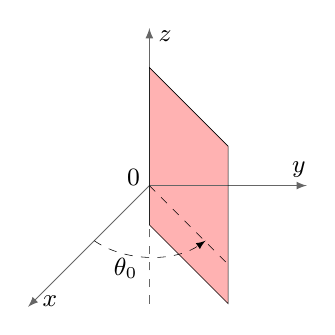
\begin{tikzpicture}
  \usetikzlibrary{arrows}
  \fill [red!30] (0,-.5) -- (1,-1.5) -- (1,.5) -- (0,1.5) -- (0,-.5);
  \draw [black!60,line width=0.3pt,-latex] (0,0) -- (2,0,0);
  \draw [black!60,line width=0.3pt,-latex] (0,-.5) -- (0,2,0);
  \draw [black!60,dashed,line width=0.3pt] (0,-1.5) -- (0,-.5);
  \draw [black!60,line width=0.3pt,-latex] (0,0) -- (0,0,4);
  \pgfputat{\pgfpointxyz{1.9}{0.2}{0}}{\pgfbox[center,center]{\small $y$}};
  \pgfputat{\pgfpointxyz{0.2}{1.9}{0}}{\pgfbox[center,center]{\small $z$}};
  \pgfputat{\pgfpointxyz{0.2}{0}{3.8}}{\pgfbox[center,center]{\small $x$}};
  \pgfputat{\pgfpointxyz{-0.2}{0.1}{0}}{\pgfbox[center,center]{\small $0$}};
  \draw [line width=0.2pt] (0,-.5) -- (1,-1.5) -- (1,.5) -- (0,1.5) -- (0,-.5);
  \draw [dashed,line width=0.2pt] (0,0) -- (1,-1);
  \draw [dashed,line width=0.2pt,-latex] (-0.7,-0.7) arc (225:315:1 and .7);
  \node [below] at (-0.3,-.8) {\small $\theta_0$};
 \end{tikzpicture}
 &
 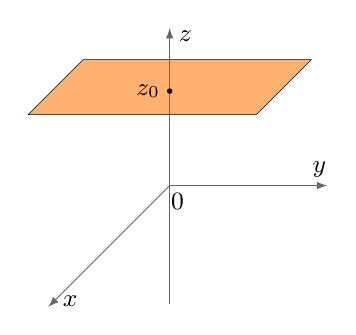
\begin{tikzpicture}
  \usetikzlibrary{arrows}
  \definecolor{planecolor}{HTML}{FFB270}
  \fill [planecolor] (-1.8,.9) -- (-1.1,1.6) -- (1.8,1.6) -- (1.1,.9) -- (-1.8,.9);
  \draw [line width=0.2pt] (-1.8,.9) -- (-1.1,1.6) -- (1.8,1.6) -- (1.1,.9) -- (-1.8,.9);
  \draw [black!60,line width=0.3pt,-latex] (0,0) -- (2,0,0);
  \draw [black!60,line width=0.3pt,-latex] (0,-1.5) -- (0,2,0);
  \draw [black!60,line width=0.3pt,-latex] (0,0) -- (0,0,4);
  \pgfputat{\pgfpointxyz{1.9}{0.2}{0}}{\pgfbox[center,center]{\small $y$}};
  \pgfputat{\pgfpointxyz{0.2}{1.9}{0}}{\pgfbox[center,center]{\small $z$}};
  \pgfputat{\pgfpointxyz{0.2}{0}{3.8}}{\pgfbox[center,center]{\small $x$}};
  \pgfputat{\pgfpointxyz{0.1}{-0.2}{0}}{\pgfbox[center,center]{\small $0$}};
  \fill (0,1.2) circle (1pt);
  \node [left] at (0,1.2) {\small $z_0$};
 \end{tikzpicture} \\
 (a) $r = r_0$ & (b) $\theta = \theta_0$ & (c) $z = z_0$
 \end{tabular}}
 \caption{Cylindrical coordinate surfaces}
 \label{fig:cylcoordsurf}
\end{lxfigure}

For spherical coordinates $(\rho,\theta,\phi)$, and constants $\rho_0$, $\theta_0$ and $\phi_0$, we see from \autoref{fig:sphcoordsurf} that the surface $\rho = \rho_0$ is a sphere of radius $\rho_0$ centered at the origin, the surface $\theta = \theta_0$ is a half-plane emanating from the $z$-axis, and the surface $\phi = \phi_0$ is a circular cone whose vertex is at the origin.

\begin{lxfigure}
 \flushinner{%
 \begin{tabular}{ccc}
 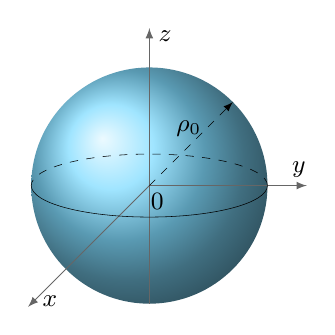
\begin{tikzpicture}
  \usetikzlibrary{arrows}
  \definecolor{spherecolor}{HTML}{80DCFF}
  \shade [ball color=spherecolor] (0,0) circle (1.5);
  \draw [black!60,line width=0.3pt,-latex] (0,0) -- (2,0,0);
  \draw [black!60,line width=0.3pt,-latex] (0,-1.5) -- (0,2,0);
  \draw [black!60,line width=0.3pt,-latex] (0,0) -- (0,0,4);
  \pgfputat{\pgfpointxyz{1.9}{0.2}{0}}{\pgfbox[center,center]{\small $y$}};
  \pgfputat{\pgfpointxyz{0.2}{1.9}{0}}{\pgfbox[center,center]{\small $z$}};
  \pgfputat{\pgfpointxyz{0.2}{0}{3.8}}{\pgfbox[center,center]{\small $x$}};
  \pgfputat{\pgfpointxyz{0.1}{-0.2}{0}}{\pgfbox[center,center]{\small $0$}};
  \draw [line width=0.2pt] (-1.5,0) arc (180:360:1.5 and 0.4);
  \draw [dashed,line width=0.2pt] (1.5,0) arc (0:180:1.5 and 0.4);
  \draw [dashed,line width=0.2pt,-latex] (0,0) -- (1.06,1.06);
  \node [above] at (0.5,0.5) {\small $\rho_0$};
 \end{tikzpicture}
 &
 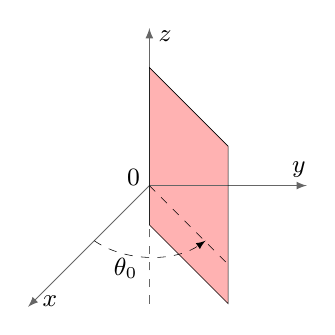
\begin{tikzpicture}
  \usetikzlibrary{arrows}
  \fill [red!30] (0,-.5) -- (1,-1.5) -- (1,.5) -- (0,1.5) -- (0,-.5);
  \draw [black!60,line width=0.3pt,-latex] (0,0) -- (2,0,0);
  \draw [black!60,line width=0.3pt,-latex] (0,-.5) -- (0,2,0);
  \draw [black!60,dashed,line width=0.3pt] (0,-1.5) -- (0,-.5);
  \draw [black!60,line width=0.3pt,-latex] (0,0) -- (0,0,4);
  \pgfputat{\pgfpointxyz{1.9}{0.2}{0}}{\pgfbox[center,center]{\small $y$}};
  \pgfputat{\pgfpointxyz{0.2}{1.9}{0}}{\pgfbox[center,center]{\small $z$}};
  \pgfputat{\pgfpointxyz{0.2}{0}{3.8}}{\pgfbox[center,center]{\small $x$}};
  \pgfputat{\pgfpointxyz{-0.2}{0.1}{0}}{\pgfbox[center,center]{\small $0$}};
  \draw [line width=0.2pt] (0,-.5) -- (1,-1.5) -- (1,.5) -- (0,1.5) -- (0,-.5);
  \draw [dashed,line width=0.2pt] (0,0) -- (1,-1);
  \draw [dashed,line width=0.2pt,-latex] (-0.7,-0.7) arc (225:315:1 and .7);
  \node [below] at (-0.3,-.8) {\small $\theta_0$};
 \end{tikzpicture}
 &
 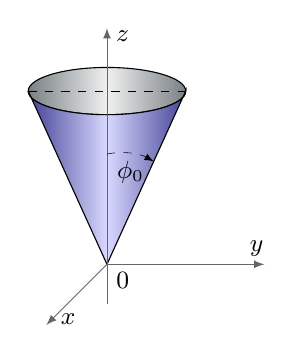
\begin{tikzpicture}
  \usetikzlibrary{arrows}
  \definecolor{insideo}{HTML}{798084}
  \definecolor{insidei}{HTML}{F0F0F0}
  \definecolor{outer}{HTML}{424296}
  \definecolor{inner}{HTML}{D8D8FF}
  \shadedraw [left color=insideo,right color=insideo,middle color=insidei] (1,2.2) arc (0:180:1 and .3) --
   (-1,2.2) arc (180:360:1 and .3);
  \shadedraw [left color=outer,right color=outer,middle color=inner] (-1,2.2) arc (180:360:1 and .3) -- (0,0) --
   (-1,2.2);
  \draw [black!60,line width=0.3pt,-latex] (0,0) -- (2,0,0);
  \draw [black!60,line width=0.3pt,-latex] (0,-.5) -- (0,3,0);
  \draw [black!60,line width=0.3pt,-latex] (0,0) -- (0,0,2);
  \pgfputat{\pgfpointxyz{1.9}{0.2}{0}}{\pgfbox[center,center]{\small $y$}};
  \pgfputat{\pgfpointxyz{0.2}{2.9}{0}}{\pgfbox[center,center]{\small $z$}};
  \pgfputat{\pgfpointxyz{0.2}{0}{1.8}}{\pgfbox[center,center]{\small $x$}};
  \pgfputat{\pgfpointxyz{0.2}{-0.2}{0}}{\pgfbox[center,center]{\small $0$}};
  \draw [dashed,line width=0.2pt] (-1,2.2) -- (1,2.2);
  \draw [dashed,line width=0.2pt,-latex] (0,1.4) arc (100:65:1 and 1.2);
  \node [above] at (0.3,0.9) {\small $\phi_0$};
 \end{tikzpicture} \\
  (a) $\rho = \rho_0$ & (b) $\theta = \theta_0$ & (c) $\phi = \phi_0$
  \end{tabular}}
 \caption{Spherical coordinate surfaces}
 \label{fig:sphcoordsurf}
\end{lxfigure}

Figures \ref{fig:cylcoordsurf}(a) and \ref{fig:sphcoordsurf}(a) show how these coordinate systems got their names.

Sometimes the equation of a surface in Cartesian coordinates can be transformed into a simpler equation in some other coordinate system, as in the following example.

\example{ex_conv_coord_eq}{Converting an Equation in Coordinate Systems}{Write the equation of the cylinder $x^2 + y^2 = 4$ in cylindrical coordinates.}{Since $r = \sqrt{x^2 + y^2}$, then the equation in cylindrical coordinates is $r =2$.}

Using spherical coordinates to write the equation of a sphere does not necessarily make the equation simpler, if the sphere is not centered at the origin.

\example{ex_bad_sphere}{Converting an Equation to Spherical Coordinates}{Write the equation $(x-2)^2+(y-1)^2+z^2=9$ in spherical coordinates.}{Multiplying the equation out gives
 \begin{align*}
  x^2+y^2+z^2-4x-2y+5 &= 9 \text{ , so we get} \\
  \rho^2-4\rho\sin\phi\cos\theta-2\rho\sin\phi\sin\theta-4 &= 0 \text{ , or}\\
  \rho^2-2\sin\phi(2\cos\theta-\sin\theta)\rho-4 &= 0
 \end{align*}
 after combining terms. Note that this actually makes it more difficult to figure out what the surface is, as opposed to the Cartesian equation where you could immediately identify the surface as a sphere of radius $3$ centered at $(2,1,0)$.}

\example{exmp_helicoid}{Identifying a Surface}{Describe the surface given by $\theta = z$ in cylindrical coordinates.}{This surface is called a \emph{helicoid}\index{helicoid}. As the (vertical) $z$ coordinate increases, so does the angle $\theta$, while the radius $r$ is unrestricted. So this sweeps out a (ruled!) surface shaped like a spiral staircase, where the spiral has an infinite radius. \autoref{fig:helicoid} shows a section of this surface restricted to $0 \le z \le 4\pi$ and $0 \le r \le 2$.
 \begin{lxfigure}
  \begin{center}
   \begin{tikzpicture}[scale=1.3]
    \begin{axis}[width=\textwidth,tick label style={font=\scriptsize},axis on top,
				axis lines=center,y dir=reverse,name=myplot,
				ymin=-2,ymax=2,xmin=-2,xmax=2,zmin=0,zmax=14]
     \addplot3[domain=0:2,y domain=0:720,surf,colormap={mp2}{\colormapplaneone},
		opacity=.6,faceted color=black!40,samples=8,samples y=72,very thin,
		z buffer=sort]
		({x*sin(y)},{x*cos(y)},{rad(y)});
    \end{axis}
    \node [left] at (myplot.below origin) [shift={(-60pt,0pt)}] {$x$};
    \node [below left] at (myplot.right of origin) [shift={(-30pt,-16pt)}] {$y$};
    \node [below] at (myplot.above origin) [shift={(0,-40pt)}] {$z$};
   \end{tikzpicture}
  \end{center}
 \caption{Helicoid $\theta = z$}\eoehere
 \label{fig:helicoid}
 \end{lxfigure}}

\printexercises{exercises/10_Other_Systems_exercises}
